% !TEX root = ../main.tex

% Section 4 — Architectural Design

\section{Architectural Design}

\subsection{Architectural style}

Room4U uses a client–server architecture with a layered modular monolith (ADR-001). The browser provides the user interface, while a single application API controls access to business operations and a PostgreSQL database stores the application data.\par

Within the API, HTTP controllers handle routing, input DTOs and response translation. Access-control components establish the authenticated actor and application role. Application services coordinate use cases, domain objects and policies enforce business rules, and persistence components execute database operations. Domain rules do not depend on browser controls, Express request objects or SQL statements.\par

This structure supports the main design goals. Centralized role and ownership checks support NFR-02. A shared transactional boundary supports conflict prevention in FR-16 and consistent rollback in NFR-09. Separating HTTP handling, business rules and persistence allows these areas to be reviewed and changed with less impact on one another. The deployment remains manageable for the four-member team and the PA1 schedule.\par

The main trade-offs are additional interfaces between layers and a shared deployment lifecycle for the API modules. The initial deployment also provides no automatic failover. Performance and recovery must therefore be evaluated against the PA2 targets; the architectural choice alone does not demonstrate that those targets have been met.\par

\subsection{System context diagram}

\begin{center}

\begin{minipage}{0.96\textwidth}

\centering

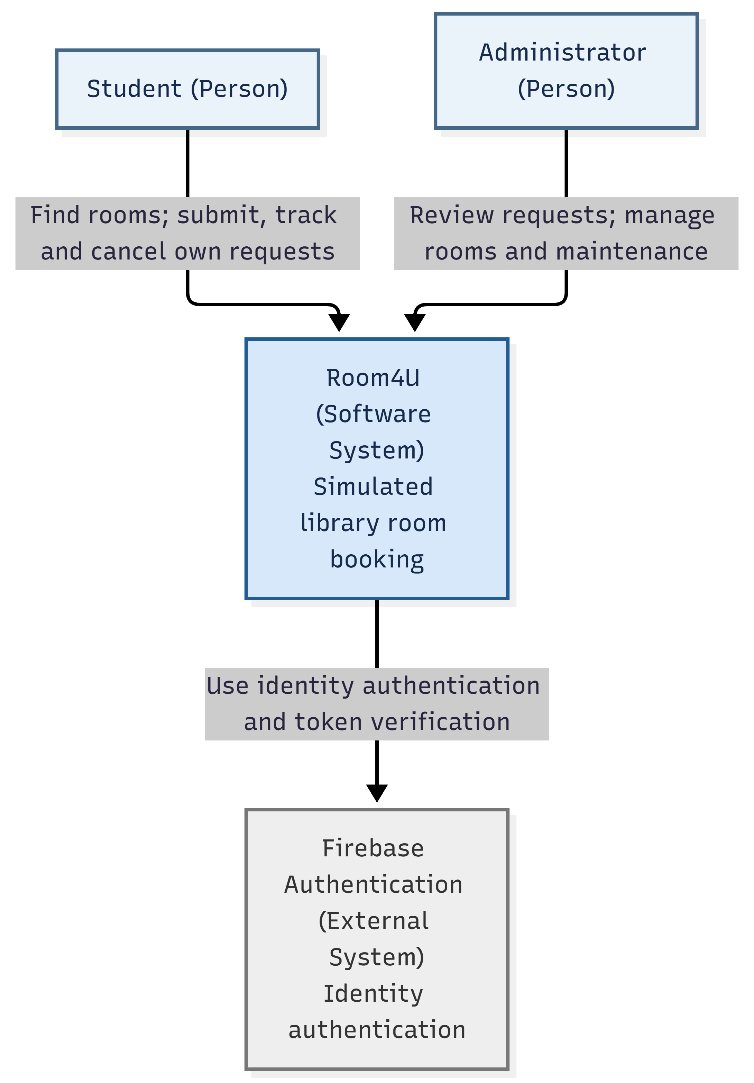
\includegraphics[width=\textwidth,height=0.62\textheight,keepaspectratio]{images/04-architectural-design-assets/architecture-figure-4.png}

\par\vspace{0.45em}

\emph{\textbf{Figure 4.2.} A01 C4 level 1. Room4U is the system boundary; its database is internal. Firebase supports identity only.}\par

\end{minipage}

\end{center}

\vspace{0.6em}



Students find rooms and manage only their own requests. Administrators process requests and manage rooms/maintenance. Instructors and the TA evaluate the coursework; they are not booking actors. Room4U does not contact the real university booking system.\par

\subsection{Container diagram}

\begin{center}

\begin{minipage}{0.96\textwidth}

\centering

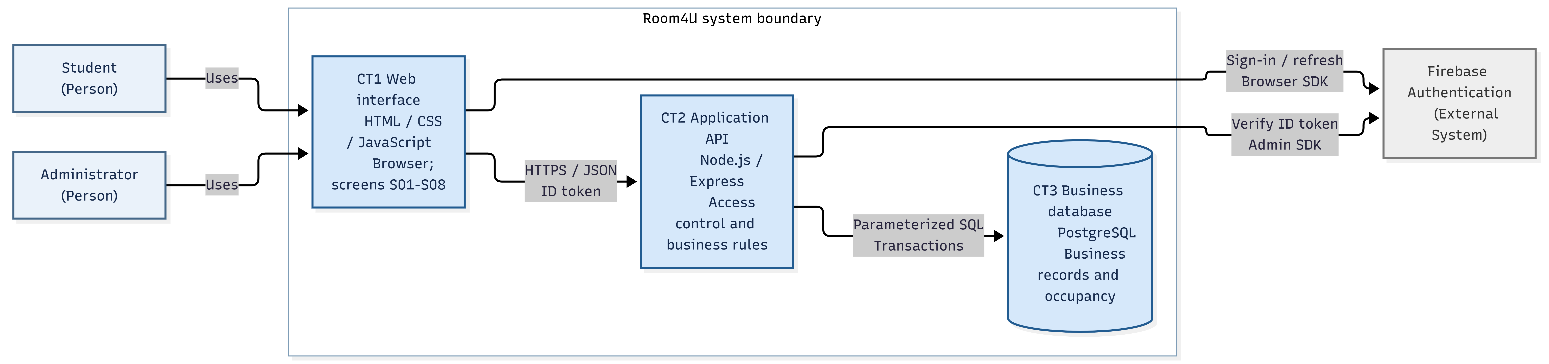
\includegraphics[width=\textwidth,height=0.62\textheight,keepaspectratio]{images/04-architectural-design-assets/architecture-figure-3.png}

\par\vspace{0.45em}

\emph{\textbf{Figure 4.3.} A02 C4 level 2. CT1 is browser JavaScript, CT2 the application API and CT3 the business database.}\par

\end{minipage}

\end{center}

\vspace{0.6em}



\begin{longtable}{|p{0.190\textwidth}|p{0.350\textwidth}|p{0.350\textwidth}|}

\hline

\textbf{Container} & \textbf{Responsibility} & \textbf{Technology and boundary} \\ \hline

\endfirsthead

\hline

\textbf{Container} & \textbf{Responsibility} & \textbf{Technology and boundary} \\ \hline

\endhead

CT1 Web interface & Render S01–S08; assist input; send authenticated commands.\allowbreak{} & HTML/\allowbreak{}CSS/\allowbreak{}Java\allowbreak{}Script; Firebase browser SDK; no authoritative rule decision.\allowbreak{} \\ \hline

CT2 Application API & Enforce roles/\allowbreak{}ownership/\allowbreak{}rules, transactions and safe DTOs.\allowbreak{} & Node.\allowbreak{}js/\allowbreak{}Express; Firebase Admin SDK; parameterized SQL through a pool.\allowbreak{} \\ \hline

CT3 Database & Persist business records and shared occupancy constraint.\allowbreak{} & Postgre\allowbreak{}SQL with btree\_\allowbreak{}gist; available only to the API/\allowbreak{}migration operator.\allowbreak{} \\ \hline

\end{longtable}

\vspace{2mm}

\subsection{Component decomposition}

\begin{center}

\begin{minipage}{0.96\textwidth}

\centering

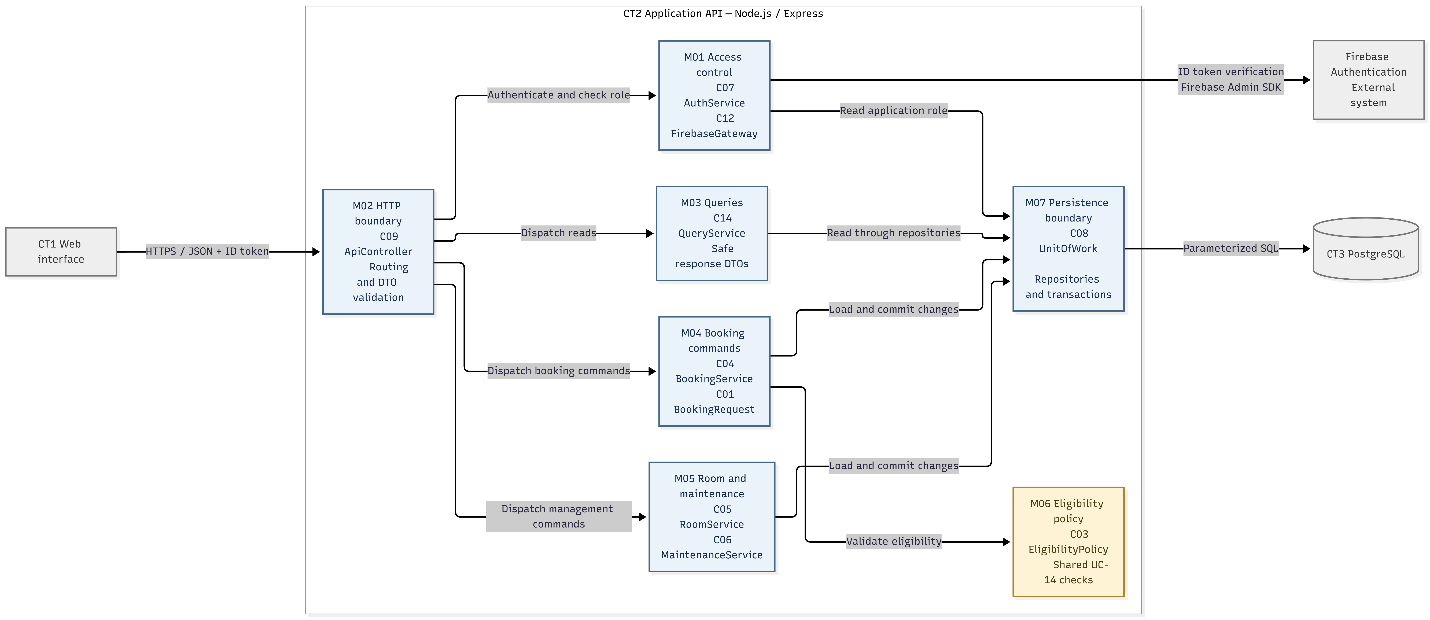
\includegraphics[width=\textwidth,height=0.62\textheight,keepaspectratio]{images/04-architectural-design-assets/architecture-figure-2.png}

\par\vspace{0.45em}

\emph{\textbf{Figure 4.4.} A03 Components inside CT2. M02 invokes access control before dispatching queries or commands.}\par

\end{minipage}

\end{center}

\vspace{0.6em}



\begin{longtable}{|p{0.190\textwidth}|p{0.350\textwidth}|p{0.350\textwidth}|}

\hline

\textbf{ID} & \textbf{Component responsibility} & \textbf{Related classes} \\ \hline

\endfirsthead

\hline

\textbf{ID} & \textbf{Component responsibility} & \textbf{Related classes} \\ \hline

\endhead

M01 & Verify identity and role; deny unauthorized access.\allowbreak{} & C07 Auth\allowbreak{}Service; C12 Firebase\allowbreak{}Gateway \\ \hline

M02 & HTTP routing, DTO validation and domain-\allowbreak{}error translation.\allowbreak{} & C09 Api\allowbreak{}Controller \\ \hline

M03 & Search, safe calendar DTO, owned history and admin queue.\allowbreak{} & C14 Query\allowbreak{}Service; read repositories \\ \hline

M04 & Submit/\allowbreak{}approve/\allowbreak{}reject/\allowbreak{}cancel with history.\allowbreak{} & C04 Booking\allowbreak{}Service; C01 Booking\allowbreak{}Request \\ \hline

M05 & Room details/\allowbreak{}state and maintenance commands.\allowbreak{} & C05 Room\allowbreak{}Service; C06 Maintenance\allowbreak{}Service; C02; C10 \\ \hline

M06 & Common UC-\allowbreak{}14 eligibility checks without writes.\allowbreak{} & C03 Eligibility\allowbreak{}Policy \\ \hline

M07 & One-\allowbreak{}client transaction, room guard, repositories and projections.\allowbreak{} & C08 Unit\allowbreak{}Of\allowbreak{}Work \\ \hline

\end{longtable}

\vspace{2mm}

M02 invokes M01 to establish the authenticated actor and check the required application role before dispatching a protected operation. Resource-specific ownership checks are performed after the requested record is loaded and before its data is returned or changed.\par

Read operations are dispatched to M03, which uses read repositories and returns explicitly selected DTO fields. Booking commands are dispatched to M04; room and maintenance commands are dispatched to M05. M04 invokes M06 for the shared UC-14 eligibility checks used by submission and approval. Command services use M07 to load current decision data and commit the complete set of changes within one transaction.\par

The component diagram shows dependencies between modules. The transaction order for state-changing operations is defined in Section 4.6.\par

\subsection{Deployment design}

\begin{center}

\begin{minipage}{0.96\textwidth}

\centering

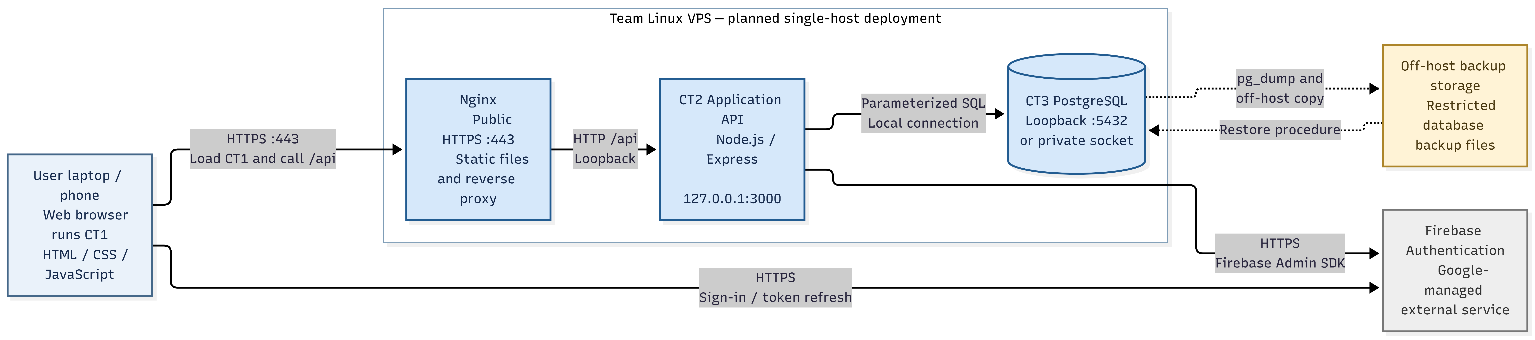
\includegraphics[width=\textwidth,height=0.62\textheight,keepaspectratio]{images/04-architectural-design-assets/architecture-figure-1.png}

\par\vspace{0.45em}

\emph{\textbf{Figure 4.5.} A04 Proposed deployment. Public access terminates at Nginx; API and database listen on private interfaces.}\par

\end{minipage}

\end{center}

\vspace{0.6em}



Nginx serves static assets and reverse-proxies /api to Express over loopback. PostgreSQL is not publicly exposed. Use one same-origin HTTPS site, explicit environment configuration and a restricted service account. Firebase credentials remain outside Git. The frontend uses Firebase-managed session state rather than copying full tokens into custom persistent storage.\par

Before PA5 demonstration: provision a clean database, apply reviewed migrations, seed test identities/roles and eight rooms, verify token handling, start the API behind Nginx and inspect a smoke path. Take a restricted database backup, copy it off-host and record the backup point. The restore drill must compare room/request/event IDs and counts and meet the PA2 recovery target. These are planned operations, not recorded successes.\par

The initial deployment places Nginx, the API and PostgreSQL on one VPS. This reduces deployment and administration work, but the host is a shared point of failure and its resources are shared by the application and database. Off-host backups support recovery; they do not provide automatic failover. The recovery procedure will be evaluated against NFR-08.\par

\subsection{Transaction protocol and schedule invariants}

\begin{longtable}{|p{0.190\textwidth}|p{0.350\textwidth}|p{0.350\textwidth}|}

\hline

\textbf{ID} & \textbf{Invariant} & \textbf{Enforcement} \\ \hline

\endfirsthead

\hline

\textbf{ID} & \textbf{Invariant} & \textbf{Enforcement} \\ \hline

\endhead

I01 & A Pending/\allowbreak{}Rejected/\allowbreak{}Cancelled request has no occupancy projection.\allowbreak{} & C04 status Change\allowbreak{}Set; C08 same-\allowbreak{}client transaction.\allowbreak{} \\ \hline

I02 & An Approved request has exactly one occupancy row matching its room and interval.\allowbreak{} & Unique booking source; composite FK; central command protocol.\allowbreak{} \\ \hline

I03 & An active maintenance block has one matching occupancy row; a removed block has none.\allowbreak{} & Unique maintenance source; composite FK; C06 create/\allowbreak{}remove transaction.\allowbreak{} \\ \hline

I04 & No two room\_\allowbreak{}occupancy intervals overlap for the same room.\allowbreak{} & Gi\allowbreak{}ST exclusion on room\_\allowbreak{}id and half-\allowbreak{}open tstzrange.\allowbreak{} \\ \hline

I05 & A capacity edit preserves all future Approved group sizes.\allowbreak{} & Same persistent room guard for capacity save and approval; current reread.\allowbreak{} \\ \hline

I06 & Every successful booking creation/\allowbreak{}transition adds one event; refused commands add none.\allowbreak{} & Request/\allowbreak{}status/\allowbreak{}occupancy/\allowbreak{}event commit or rollback together.\allowbreak{} \\ \hline

I07 & Suspension blocks subsequent submission/\allowbreak{}approval, not existing occupancy.\allowbreak{} & Room state rechecked inside the guard; retain source/\allowbreak{}projection rows.\allowbreak{} \\ \hline

I08 & Public calendar data contains availability without another student identity.\allowbreak{} & M03 explicit DTO allowlist; detail routes enforce owner/\allowbreak{}Admin.\allowbreak{} \\ \hline

\end{longtable}

\vspace{2mm}

All commands affecting an existing room use this order: authorize the actor; obtain the target room ID without exposing protected data; BEGIN at READ COMMITTED; SELECT the persistent rooms row FOR UPDATE; load the current target and occupancy; capture server decision time; validate; save the complete ChangeSet; COMMIT; then return success. If any step fails, ROLLBACK and release the same pool client. Creating a new room is the only command without an existing room guard; normalized code uniqueness is enforced by PostgreSQL.\par

Use a fresh UnitOfWork for each command. Never share a checked-out client between concurrent requests, and never perform Firebase calls while holding the room lock. All booking/maintenance/state/capacity writers must follow this protocol, including future API instances. If a command ever spans several rooms, acquire room IDs in sorted order; no such operation is currently exposed.\par

Locking only overlapping booking rows is insufficient when no matching row exists. The room row is a stable guard even for an empty schedule. PostgreSQL row locks hold until transaction end [R1]. The database exclusion constraint adds protection across both booking and maintenance projections [R2]. I01–I03 and event correspondence also depend on the centralized transaction writer; the exclusion constraint alone does not prove them.\par

After waiting for the room lock, validation queries run as subsequent READ COMMITTED statements and therefore see committed preceding room writes [R5]. The injected decision clock is sampled after that wait, not from a transaction-start timestamp. In PostgreSQL use a fresh clock\_timestamp() result (or equivalent server clock) for the decision; reject non-finite timestamps and start values with nonzero seconds/subseconds. Local-hour and same-date checks use Asia/Ho\_Chi\_Minh.\par

Lock order is room row first, then the target request/block if a separate record lock is needed. A database lock timeout is an operational failure, not proof that the room is booked. An unknown commit outcome is reconciled by reading the resource or replaying the original submission key; the client must not create a new key automatically.\par

\subsubsection{Race outcomes to preserve}

\begin{longtable}{|p{0.190\textwidth}|p{0.350\textwidth}|p{0.350\textwidth}|}

\hline

\textbf{Concurrent actions} & \textbf{Permitted outcome} & \textbf{Refusal behavior} \\ \hline

\endfirsthead

\hline

\textbf{Concurrent actions} & \textbf{Permitted outcome} & \textbf{Refusal behavior} \\ \hline

\endhead

Two overlapping approvals & One commits; the second rechecks and finds occupancy.\allowbreak{} & Second stays Pending; no new event.\allowbreak{} \\ \hline

Approval vs maintenance creation & The first valid command occupies the interval.\allowbreak{} & Second refuses overlap; never both occupied.\allowbreak{} \\ \hline

Approval vs suspension & Approval first: booking retained.\allowbreak{} Suspension first: new approval denied.\allowbreak{} & No automatic cancellation.\allowbreak{} \\ \hline

Approval vs capacity reduction & Approval first: capacity save checks its group.\allowbreak{} Edit first: approval uses new capacity.\allowbreak{} & Unsafe action refused; invariant I05 holds.\allowbreak{} \\ \hline

Owner cancel vs approval & Room guard orders decisions.\allowbreak{} Cancelled cannot later be approved.\allowbreak{} & If state changed, report current outcome; no duplicate event.\allowbreak{} \\ \hline

Removal vs passage of start time & Removal checks active state and decision time after the guard.\allowbreak{} & At/\allowbreak{}after start, refuse removal and retain occupancy.\allowbreak{} \\ \hline

Repeated command /\allowbreak{} lost response & A creation replay reuses owner/\allowbreak{}submission\allowbreak{}Key; decisions reread state.\allowbreak{} & Never infer success from a timeout; refresh authoritative state.\allowbreak{} \\ \hline

\end{longtable}

\vspace{2mm}

C08 implements this shared transaction boundary for every room command. The schema example and full proposed SQL source are described in Section 6. Validation, authorization and rollback paths remain part of each service operation.\par

\subsection{Architecture Decision Records}

The following ADRs document the proposed architectural decisions, their context, alternatives and consequences. Their current status is Accepted. Each ADR is to be maintained as a separate record under docs/design/adr/, consistent with the PA3 template.\par

\subsubsection{ADR-001 Use a layered modular monolith}

\begin{longtable}{|p{0.200\textwidth}|p{0.740\textwidth}|}

\hline

\textbf{Field} & \textbf{Record} \\ \hline

\endfirsthead

\hline

\textbf{Field} & \textbf{Record} \\ \hline

\endhead

Status & Accepted \\ \hline

Context & Four students must implement five feature groups within the PA1 schedule.\allowbreak{} Booking and availability changes need one reliable transactional boundary.\allowbreak{} \\ \hline

Decision & Use a browser client and one Express deployment.\allowbreak{} Separate HTTP/\allowbreak{}access control, queries, command services, domain policies and persistence.\allowbreak{} Keep the application tables in one Postgre\allowbreak{}SQL database; ADR-\allowbreak{}005 refines the model to seven tables.\allowbreak{} \\ \hline

Alternatives considered & Microservices: adds distributed authorization, deployment and consistency work.\allowbreak{} A single unstructured Express file: initially shorter but mixes rules, HTTP and SQL.\allowbreak{} \\ \hline

Consequences & The design provides a small deployment and a local transaction boundary for booking decisions.\allowbreak{} Separating responsibilities allows services and policies to be verified through injected dependencies.\allowbreak{} Module boundaries must be maintained during implementation and code review.\allowbreak{} API modules are deployed together, and the initial single-\allowbreak{}instance deployment provides no automatic failover.\allowbreak{} Application and database resource usage must be evaluated on the PA1 reference environment before claiming compliance with the PA2 performance targets.\allowbreak{} \\ \hline

\end{longtable}

\vspace{2mm}

\subsubsection{ADR-002 Serialize room writes and share one occupancy constraint}

\begin{longtable}{|p{0.200\textwidth}|p{0.740\textwidth}|}

\hline

\textbf{Field} & \textbf{Record} \\ \hline

\endfirsthead

\hline

\textbf{Field} & \textbf{Record} \\ \hline

\endhead

Status & Accepted \\ \hline

Context & Two approvals, maintenance creation, suspension and capacity edits must make consistent decisions even when the room initially has no occupied interval.\allowbreak{} \\ \hline

Decision & At READ COMMITTED, lock the persistent rooms row before loading current decision data.\allowbreak{} Use the same lock for every command affecting that room.\allowbreak{} Represent Approved bookings and active maintenance in room\_\allowbreak{}occupancy, protected by a room/\allowbreak{}range Gi\allowbreak{}ST exclusion constraint.\allowbreak{} \\ \hline

Alternatives considered & Check then write without a lock: both requests can pass.\allowbreak{} Lock only overlapping booking rows: locks no guard when the set is empty.\allowbreak{} An in-\allowbreak{}memory mutex: does not protect another API process.\allowbreak{} SERIALIZABLE with retries: viable, but more retry handling than the selected explicit room guard.\allowbreak{} \\ \hline

Consequences & Different rooms can progress concurrently; writes for one room wait for each other.\allowbreak{} The occupancy projection adds transactional maintenance work and btree\_\allowbreak{}gist must be available.\allowbreak{} Centralized write paths, source foreign keys and rollback checks are required.\allowbreak{} Validate the migration and races in PA5.\allowbreak{} \\ \hline

\end{longtable}

\vspace{2mm}

\subsubsection{ADR-003 Use Firebase identity with application role checks}

\begin{longtable}{|p{0.200\textwidth}|p{0.740\textwidth}|}

\hline

\textbf{Field} & \textbf{Record} \\ \hline

\endfirsthead

\hline

\textbf{Field} & \textbf{Record} \\ \hline

\endhead

Status & Accepted \\ \hline

Context & PA1 uses Firebase Authentication and pre-\allowbreak{}created accounts.\allowbreak{} Room4U still owns Student/\allowbreak{}Admin permissions and request ownership; there is no university SSO integration.\allowbreak{} \\ \hline

Decision & Use the Firebase browser SDK for email/\allowbreak{}password sign-\allowbreak{}in.\allowbreak{} The API verifies bearer ID tokens through Firebase Admin SDK, looks up firebase\_\allowbreak{}uid in users and derives the role from that database row.\allowbreak{} The browser cannot supply a trusted role or owner ID.\allowbreak{} \\ \hline

Alternatives considered & A custom password database: unnecessary credential-\allowbreak{}handling work.\allowbreak{} Client-\allowbreak{}side role checks only: bypassable.\allowbreak{} University SSO: outside the committed scope.\allowbreak{} \\ \hline

Consequences & Passwords do not enter the Room4U API or database.\allowbreak{} Identity verification depends on Firebase configuration and network/\allowbreak{}key availability.\allowbreak{} Sign-\allowbreak{}out clears local identity/\allowbreak{}private views; it does not promise revocation of a copied token.\allowbreak{} No public registration or recovery screen is added.\allowbreak{} \\ \hline

\end{longtable}

\vspace{2mm}

\subsubsection{ADR-004 Keep time policy centralized and retries explicit}

\begin{longtable}{|p{0.200\textwidth}|p{0.740\textwidth}|}

\hline

\textbf{Field} & \textbf{Record} \\ \hline

\endfirsthead

\hline

\textbf{Field} & \textbf{Record} \\ \hline

\endhead

Status & Accepted \\ \hline

Context & Booking rules use local library hours, a rolling seven-\allowbreak{}day limit and duration input.\allowbreak{} Stale schedules and lost responses must not be interpreted as successful decisions.\allowbreak{} \\ \hline

Decision & Store instants as timestamptz, display Asia/\allowbreak{}Ho\_\allowbreak{}Chi\_\allowbreak{}Minh, and derive end\allowbreak{}At from start plus duration.\allowbreak{} Evaluate decision time after obtaining the room lock.\allowbreak{} Use stable error codes and a client-\allowbreak{}generated submission key for each logical create-\allowbreak{}request command.\allowbreak{} \\ \hline

Alternatives considered & Store local timestamp strings: ambiguous comparisons.\allowbreak{} Accept end time as an independent booking input: changes the current PA2 form.\allowbreak{} Blindly retry POST with a new key: can create duplicate requests.\allowbreak{} \\ \hline

Consequences & The clock can be fixed for boundary verification.\allowbreak{} The submission key is a technical retry mechanism, not a new booking feature.\allowbreak{} Same owner/\allowbreak{}key and same payload returns the existing request; a reused key with different input is refused.\allowbreak{} Implementation must preserve these agreed time and replay semantics across the API, persistence and user interface.\allowbreak{} \\ \hline

\end{longtable}

\vspace{2mm}

\subsubsection{ADR-005: UI-Data Contracts}

\begin{longtable}{|p{0.200\textwidth}|p{0.740\textwidth}|}

\hline

\textbf{Field} & \textbf{Record} \\ \hline

\endfirsthead

\hline

\textbf{Field} & \textbf{Record} \\ \hline

\endhead

Status & Accepted \\ \hline

Context & PA2 S03 uses a required purpose dropdown and an optional note with a 250-\allowbreak{}character counter.\allowbreak{} S04 and S06 display requester profile fields missing from the initial PA3 schema.\allowbreak{} S02 and S07 use equipment checkboxes.\allowbreak{} The leader chooses to retain requester profiles and equipment selection, while removing the separate related-\allowbreak{}course field and room-\allowbreak{}area information.\allowbreak{} \\ \hline

Decision & Use stable purpose codes validated by the API and database, with Vietnamese UI labels defined below.\allowbreak{} Add full\_\allowbreak{}name, student\_\allowbreak{}code and phone to pre-\allowbreak{}created users.\allowbreak{} Keep purpose required and note optional with a 250-\allowbreak{}character limit.\allowbreak{} Remove related-\allowbreak{}course and area controls and displays.\allowbreak{} Represent room equipment in room\_\allowbreak{}equipment rather than an editable delimited description in rooms.\allowbreak{} Use the shared catalogues below across UI, API, seeds and persistence.\allowbreak{} \\ \hline

Alternatives considered & Unrestricted purpose text preserves flexibility but does not define the dropdown contract.\allowbreak{} Storing translated labels makes stored values depend on presentation wording.\allowbreak{} Removing supported profile fields would reduce the PA2 interface unnecessarily.\allowbreak{} Parsing equipment descriptions to reconstruct checkboxes makes selection and filtering ambiguous.\allowbreak{} Adding editable purpose/\allowbreak{}equipment catalogues creates management work outside the current scope.\allowbreak{} \\ \hline

Consequences & The proposed model has seven tables.\allowbreak{} UI dropdowns, checkbox values, API DTOs, database checks and seed data must remain synchronized.\allowbreak{} Labels may change without rewriting stable codes.\allowbreak{} Changing the code catalogue requires a reviewed design/\allowbreak{}schema update.\allowbreak{} Equipment joins add persistence work but provide explicit selections and filters.\allowbreak{} This refines the data representation in ADR-\allowbreak{}001 without changing its modular-\allowbreak{}monolith decision.\allowbreak{} \\ \hline

\end{longtable}

\vspace{2mm}

\subsubsection{Purpose catalogue}

\begin{longtable}{|p{0.200\textwidth}|p{0.740\textwidth}|}

\hline

\textbf{Stored/\allowbreak{}API code} & \textbf{Vietnamese UI label} \\ \hline

\endfirsthead

\hline

\textbf{Stored/\allowbreak{}API code} & \textbf{Vietnamese UI label} \\ \hline

\endhead

GROUP\_\allowbreak{}STUDY & Học nhóm \\ \hline

PROJECT\_\allowbreak{}DISCUSSION & Thảo luận đồ án \\ \hline

ASSIGNMENT\_\allowbreak{}WORK & Làm bài tập \\ \hline

ACADEMIC\_\allowbreak{}RESEARCH & Nghiên cứu học tập \\ \hline

OTHER & Hoạt động học tập khác \\ \hline

\end{longtable}

\vspace{2mm}

Purpose is required. The API and database accept only the listed codes. Selecting OTHER does not make the optional note mandatory. Purpose does not introduce approval priority or a new purpose-based eligibility condition.\par

\subsubsection{Equipment catalogue}

\begin{longtable}{|p{0.200\textwidth}|p{0.740\textwidth}|}

\hline

\textbf{Stored/\allowbreak{}API code} & \textbf{Vietnamese UI label} \\ \hline

\endfirsthead

\hline

\textbf{Stored/\allowbreak{}API code} & \textbf{Vietnamese UI label} \\ \hline

\endhead

WHITEBOARD & Bảng trắng \\ \hline

DISPLAY\_\allowbreak{}SCREEN & Màn hình /\allowbreak{} TV \\ \hline

POWER\_\allowbreak{}OUTLET & Ổ cắm điện \\ \hline

AIR\_\allowbreak{}CONDITIONER & Điều hòa \\ \hline

WIFI & Wi-\allowbreak{}Fi \\ \hline

\end{longtable}

\vspace{2mm}

Each selected equipment checkbox corresponds to one room\_equipment row. An empty selection produces no equipment rows for the room. Multiple equipment filters use AND semantics: the room must contain every selected code. Display descriptions are generated from the shared labels rather than stored as a second editable equipment value.\par

\subsubsection{Submission replay and database error handling}

Before the first submission, CT1 generates a submissionKey for the logical create-request command and retains it when retrying an unchanged submission after a lost response.\par

After authenticating the actor, the API checks whether a request already exists for the same owner and submissionKey. If its original submitted values match, the API returns the existing request with its current status and HTTP 200 without creating another request, occupancy row or creation event. This replay is not evaluated as a new booking submission. Reusing the key with different submitted values returns HTTP 409.\par

If the first lookup finds no request, the API begins the transaction, obtains the room guard and then looks up the same (ownerId, submissionKey) pair again before running UC-14. If this second lookup finds a request, the transaction is rolled back and the stored request is compared with the submitted values: an identical replay returns the current record with HTTP 200, while different values return HTTP 409. Only when the second lookup also finds no request does the API run UC-14 and continue the normal submission transaction protocol. A unique constraint on (ownerId, submissionKey) handles concurrent submissions, including submissions targeting different rooms. If insert encounters that unique constraint, the transaction is rolled back before the stored request is reread and compared; matching data returns the existing record with HTTP 200 and different data returns HTTP 409.\par

SQLSTATE 23P01 is translated into an overlap conflict. SQLSTATE 23505 is interpreted using the violated named constraint. Any retry after a deadlock or serialization failure starts a new transaction and rereads the current decision data.\par

\subsection{API and data transfer contracts}

All business routes are under /api/v1. Actor means server-injected AuthContext, never a trusted userId/role from request JSON. Firebase email/password exchange happens between browser SDK and Firebase; Room4U does not expose a password-taking login API. Sign-out is a browser session operation, followed by protected-route checks on later access.\par

\begin{longtable}{|p{0.160\textwidth}|p{0.150\textwidth}|p{0.190\textwidth}|p{0.400\textwidth}|}

\hline

\textbf{Route} & \textbf{Permission} & \textbf{Design operation} & \textbf{Contract} \\ \hline

\endfirsthead

\hline

\textbf{Route} & \textbf{Permission} & \textbf{Design operation} & \textbf{Contract} \\ \hline

\endhead

GET /\allowbreak{}me & Both & C09.\allowbreak{}me & C07.\allowbreak{}authorize runs first to authenticate and issue Auth\allowbreak{}Context. C09.\allowbreak{}me returns id, email, full\allowbreak{}Name, role and permitted own-\allowbreak{}profile fields student\allowbreak{}Code/\allowbreak{}phone. No password/\allowbreak{}token echo. \\ \hline

GET /rooms & Both & C09.\allowbreak{}search → C14.\allowbreak{}search & Return room DTOs containing id, code, name, floor, capacity, equipment\allowbreak{}Codes, derived equipment\allowbreak{}Description, description, optional photo\allowbreak{}Ref and room state. Query filters are date, group\allowbreak{}Size and repeated optional equipment\allowbreak{}Codes. A room must contain every selected equipment code. Apply filters before pagination and result counts. Do not return another student's identity. \\ \hline

GET /\allowbreak{}rooms/\allowbreak{}:id/\allowbreak{}schedule?date= & Both & C14.\allowbreak{}schedule & Occupied intervals and type only; no request owner/\allowbreak{}reason in shared view.\allowbreak{} \\ \hline

POST /\allowbreak{}requests & Student & C04.\allowbreak{}submit & Accept room\allowbreak{}Id, start\allowbreak{}At, duration\allowbreak{}Minutes, group\allowbreak{}Size, a required purpose code defined in ADR-\allowbreak{}005, optional note of at most 250 characters, and submission\allowbreak{}Key.\allowbreak{} Derive the owner from Auth\allowbreak{}Context.\allowbreak{} Return 201 for a new request or 200 for an identical replay.\allowbreak{} \\ \hline

GET /\allowbreak{}requests/\allowbreak{}mine & Student & C14.\allowbreak{}my\allowbreak{}Requests & Owned requests only, optionally status-\allowbreak{}filtered and paginated.\allowbreak{} \\ \hline

GET /\allowbreak{}requests/\allowbreak{}:id & Owner or Admin & C14.\allowbreak{}request\allowbreak{}Detail & Return the authorized requester profile, stored purpose code, optional note and existing history.\allowbreak{} No related\allowbreak{}Course or area fields.\allowbreak{} \\ \hline

POST /\allowbreak{}requests/\allowbreak{}:id/\allowbreak{}cancel & Owner or Admin & C04.\allowbreak{}cancel & Owner: Pending/\allowbreak{}Approved before start.\allowbreak{} Admin: Approved before start plus reason.\allowbreak{} \\ \hline

GET /\allowbreak{}admin/\allowbreak{}requests?status= & Admin & C14.\allowbreak{}queue & Default Pending; includes Approved filter; stable created\allowbreak{}At/\allowbreak{}id order.\allowbreak{} \\ \hline

POST /\allowbreak{}admin/\allowbreak{}requests/\allowbreak{}:id/\allowbreak{}approve & Admin & C04.\allowbreak{}approve & Current Pending plus UC-\allowbreak{}14; 409 on conflict/\allowbreak{}stale state.\allowbreak{} \\ \hline

POST /\allowbreak{}admin/\allowbreak{}requests/\allowbreak{}:id/\allowbreak{}reject & Admin & C04.\allowbreak{}reject & Trimmed reason, Pending; past Pending can be rejected.\allowbreak{} \\ \hline

GET /admin/rooms & Admin & C09.\allowbreak{}search → C14.\allowbreak{}search & Optional q, floor, status, page and pageSize. q matches room code or name case-insensitively; status filters displayStatus. Apply filters before pagination; sort stably by room code then ID. Return the filtered page, filtered total and an unfiltered summary for all rooms with one server-selected asOf. DTOs include displayStatus: suspended rooms are suspended; active rooms with an active maintenance block where startAt $\leq$ asOf $<$ endAt are under\_maintenance; remaining active rooms are active. Summary returns total, active, underMaintenance and suspended counts using that same classification and asOf; every room belongs to exactly one group. \\ \hline

POST /\allowbreak{}admin/\allowbreak{}rooms & Admin & C05.\allowbreak{}save\allowbreak{}Room & Accept code, name, floor, capacity, equipment\allowbreak{}Codes, optional description and optional preloaded photo\allowbreak{}Ref. Blank, omitted or null photo\allowbreak{}Ref uses the default room image. Validate room-code uniqueness and field rules; save room and equipment atomically. A new room is Active. \\ \hline


PATCH /\allowbreak{}admin/\allowbreak{}rooms/\allowbreak{}:id & Admin & C05.\allowbreak{}save\allowbreak{}Room & Update editable details while preserving the room ID. Supplied equipment\allowbreak{}Codes replaces the set; omission preserves it. Omitted photo\allowbreak{}Ref preserves the current image, null clears it and uses the default, and a valid existing-image reference selects it. Save atomically under the room guard, including the future-Approved capacity check. State changes use suspend/\allowbreak{}resume routes. \\ \hline

POST /\allowbreak{}admin/\allowbreak{}rooms/\allowbreak{}:id/\allowbreak{}suspend & Admin & C05.\allowbreak{}set\allowbreak{}Room\allowbreak{}State & Confirm intent, reread state; preserve occupancy.\allowbreak{} \\ \hline

POST /\allowbreak{}admin/\allowbreak{}rooms/\allowbreak{}:id/\allowbreak{}resume & Admin & C05.\allowbreak{}set\allowbreak{}Room\allowbreak{}State & Current suspended state; preserve occupancy.\allowbreak{} \\ \hline

GET /\allowbreak{}admin/\allowbreak{}rooms/\allowbreak{}:id/\allowbreak{}maintenance & Admin & C14.\allowbreak{}maintenance & Retained block records, with active/\allowbreak{}removed state.\allowbreak{} \\ \hline

POST /\allowbreak{}admin/\allowbreak{}rooms/\allowbreak{}:id/\allowbreak{}maintenance & Admin & C06.\allowbreak{}create\allowbreak{}Maintenance & Accept start\allowbreak{}At, end\allowbreak{}At and reason. Return HTTP 409 with error.code = SCHEDULE\_CONFLICT, error.requestId and error.conflicts. Following SQ05, conflicts contains Approved bookings first when any overlap (each item: kind = approved\_booking, bookingRequestId, startAt, endAt); only when none overlap, return the conflicting active maintenance block (kind = maintenance\_block, maintenanceBlockId, startAt, endAt). No booking is cancelled automatically. \\ \hline

POST /\allowbreak{}admin/\allowbreak{}maintenance/\allowbreak{}:id/\allowbreak{}remove & Admin & C06.\allowbreak{}remove\allowbreak{}Maintenance & Current active future block; retain source and release only its projection.\allowbreak{} \\ \hline

\end{longtable}

\vspace{2mm}

Multiple equipment filters use repeated query parameters, for example equipmentCodes=WHITEBOARD\allowbreak{}\&\allowbreak{}equipmentCodes=WIFI. The API validates and de-duplicates the codes. Omitting equipmentCodes adds no equipment condition.\par

Command responses include the current resource ID/status and a request correlation ID. Errors have \{error:\{code,message,fieldErrors?,conflicts?,requestId\}\}; maintenance schedule conflicts use SCHEDULE\_CONFLICT and include error.conflicts for the Administrator. Codes are stable for the UI; Vietnamese text may change without changing control logic. A shared calendar response contains roomId, startAt, endAt and occupancy type, not owner IDs or processing reasons. Authoritative lists are paged; page size is a proposed implementation bound, not a new business limit.\par

\begin{longtable}{|p{0.190\textwidth}|p{0.350\textwidth}|p{0.350\textwidth}|}

\hline

\textbf{HTTP status} & \textbf{Meaning} & \textbf{UI reaction} \\ \hline

\endfirsthead

\hline

\textbf{HTTP status} & \textbf{Meaning} & \textbf{UI reaction} \\ \hline

\endhead

401 & Missing/\allowbreak{}invalid identity.\allowbreak{} & Clear private view and require sign-\allowbreak{}in; never loop endlessly on refresh.\allowbreak{} \\ \hline

403 & Valid identity but disallowed role/\allowbreak{}ownership.\allowbreak{} & Show access denied without protected record data.\allowbreak{} \\ \hline

404 & Unknown requested resource.\allowbreak{} & Show unavailable record; do not manufacture state.\allowbreak{} \\ \hline

409 & Current status, schedule, code or submission-\allowbreak{}key conflict.\allowbreak{} & Refresh state; preserve safe user input; require a new eligible decision.\allowbreak{} \\ \hline

422 & Malformed domain input or field constraints.\allowbreak{} & Link errors to fields; retain non-\allowbreak{}sensitive valid values.\allowbreak{} \\ \hline

503 & Unavailable persistence/\allowbreak{}identity dependency or bounded lock wait.\allowbreak{} & Show retry; do not claim commit or automatically use a new submission key.\allowbreak{} \\ \hline

\end{longtable}

\vspace{2mm}

\subsection{Interface examples and contract consistency}

The following example illustrates a new booking submission. Assume that the server decision time is 2026-11-15T09:00:00+07:00 and the selected room is Active, has sufficient capacity and has no conflicting occupancy. Identifiers are illustrative.\par

\begingroup
\small
\begin{samepage}
\begin{verbatim}
POST /api/v1/requests

{
  "roomId": "11111111-1111-4111-8111-111111111111",
  "startAt": "2026-11-16T14:00:00+07:00",
  "durationMinutes": 90,
  "groupSize": 4,
  "purpose": "GROUP_STUDY",
  "note": "Ôn tập môn Cơ sở dữ liệu",
  "submissionKey": "22222222-2222-4222-8222-222222222222"
}
\end{verbatim}
\end{samepage}
\endgroup

The server derives endAt from startAt and durationMinutes. A successful new submission returns HTTP 201 with the created request:\par

\begingroup
\small
\begin{samepage}
\begin{verbatim}
{
  "id": "33333333-3333-4333-8333-333333333333",
  "status": "Pending",
  "startAt": "2026-11-16T14:00:00+07:00",
  "endAt": "2026-11-16T15:30:00+07:00",
  "groupSize": 4,
  "requiresApproval": true
}
\end{verbatim}
\end{samepage}
\endgroup

Pending confirms that the request has been recorded for review. It does not reserve the room or create an occupancy row.\par

If a command conflicts with the current schedule, the API returns HTTP 409 using a stable error code:\par

\begingroup
\small
\begin{samepage}
\begin{verbatim}
{
  "error": {
    "code": "SCHEDULE_CONFLICT",
    "message": "Khoảng thời gian không còn phù hợp.",
    "requestId": "corr-example-001"
  }
}
\end{verbatim}
\end{samepage}
\endgroup

Authorized Administrator views may identify relevant conflicting source records. Shared Student calendars expose occupied intervals and their type without disclosing another student's identity or processing reasons.\par

API DTOs, class specifications, database fields and screen specifications must remain consistent. Booking purpose and the optional note are carried through submission and authorized request details, as described in PA2. Room details cover the information presented in the PA2 room-management prototype. Any unresolved field requiredness or length bounds must be recorded for team review before implementation; no additional business restriction is assumed.\par